\documentclass[main.tex]{subfiles}
\begin{document}

% \section*{4 October 2019}
\marginpar{Friday\\ 2019-10-4, \\ compiled \\ \today}

% From yesterday we recall that \(k=0\) iff \(\rho (t) = \rho_C(t)\).

% We can write \(H (t_0) = H_0 = 100 h \times \SI{}{\kilo\metre\per\second\per\mega\parsec} \).
% Do note that \(\SI{1}{\mega\parsec} = \SI{3.086e22}{\metre}\).

% If we have \(H\) we can find \(\rho_{0C} = h^2 \times \SI{1.88e-28}{\gram\per\cubic\metre}\). We have defined \(\Omega(t) \defeq \rho / \rho_C\): recall that \(\sign{\Omega -1} = \sign k\).

% So we want to measure the energy density in galaxies to figure out what \(\Omega\) is.

The Schechter function is an empirical estimate for the shape of this distribution:
%
\begin{equation}
  \Phi(L) = \frac{\Phi^*}{L^*} \qty(\frac{L}{L^*})^{-\alpha} \exp(-\frac{L}{L^*})
  \,,
\end{equation}
%
where \(\Phi_{*}\), \(L_{*}\) and \(\alpha \) are parameters, with dimensions of respectively a number density, a luminosity and a pure number.

These can be fit by observation: we find \(\Phi^* \approx \SI{e-2}{} h^3 \SI{}{\mega\parsec^{-3}}\), \(L^* \approx \num{e10}h^{-2} L_\odot \) and \(\alpha \approx 1\).

\begin{figure}[ht]
\centering
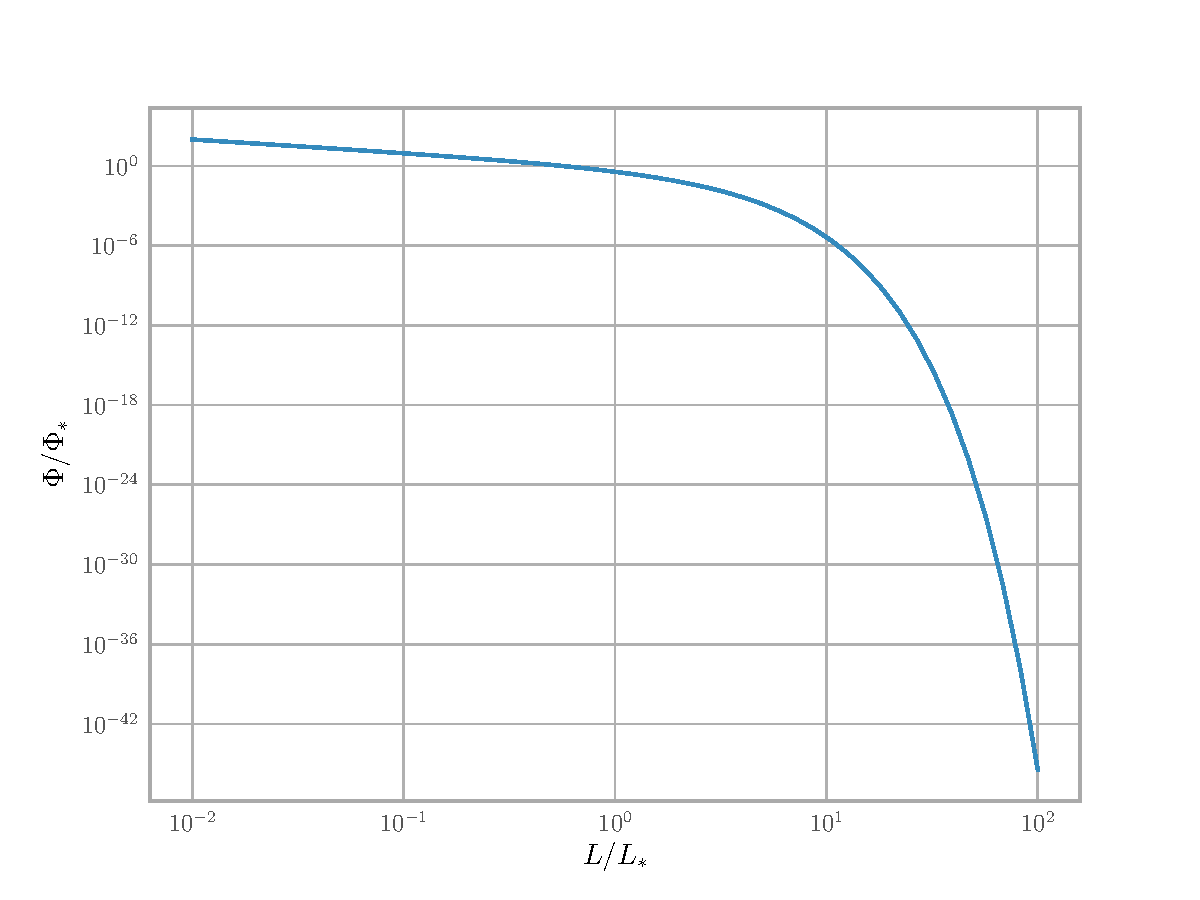
\includegraphics[width=\textwidth]{figures/Schechter.pdf}
\caption{A rough plot of the Schechter function for \(\alpha = 1\).}
\label{fig:Schechter}
\end{figure}

The integral for \(\mathscr L_g\) converges despite the divergence of \(\Phi(L)\) as \(L \rightarrow 0\), since it is multiplied by \(L\): so we do not need to really worry about the low-luminosity divergence of the distribution.

The result of the integral for a generic value of \(\alpha \) is \(\mathscr L_g = \Phi^* L^* \Gamma(2-\alpha)\), where \(\Gamma\) is the Euler gamma function; for the \(\alpha = 1\) case we get a factor \(\Gamma(2-1) = 1\).

Numerically, we get \(\mathscr{L}_{g} \approx \num{2.0(7)e8} h L_\odot \SI{}{\per\cubic\mega\parsec}. \) 
\todo[inline]{This is reported incorrectly in \cite{Pacciani:2018} as \(\sim \num{e18}\)! The correct figure can be found in \cite[eq. 4.5.14]{LucchinColes:2002}.
I do not think there is much of a point in reporting the specific value, since the parameters are already given as order-of-magnitude estimates.}

Now, we must estimate \(\expval{M / L}\).
The luminosity of galaxies can be measured readily, the great difficulty lies in estimating their mass.

\subsection{Estimating the masses of galaxies}

We must distinguish between the different shapes of the galaxies: spiral galaxies are characterized by rotation of the stars about the galactic center, while in elliptical galaxies the stars' motion is disordered.

\subsubsection{Spiral galaxies}

If we see a spiral galaxy edge-on, we will have a side of it coming in our direction, and the other side moving away from us (after correcting for other sources of Doppler shift, such as the velocity of the whole galaxy).
So, using the Doppler effect we can measure the distribution of the velocity in the galaxy as a function of the radius. 

% We plot the velocity of rotation of galaxies \(v\)  against the radius \(R\).

In order to get a theoretical model, we can approximate the galaxy as a sphere: this is very rough (spiral galaxies are closer to being disk-like), but it gives the same qualitative result, so there is no need for a more precise model in this context.

We model the galaxy velocity distribution using Newtonian mechanics: the GR corrections are negligible at these scales, galaxies are much larger than their Schwarzschild radii.

Equating the gravitational force \(GM/R^2\) to the centripetal acceleration \(v^2 /R\) we find: 
%
\begin{align}
v = \sqrt{\frac{GM}{R}}
\,,
\end{align}
%
where \(v\) and \(M\) are functions of \(R\): \(M\) is the mass contained in the spherical shell of radius \(R\), and \(v\) is the orbital velocity at the boundary of the shell.

In the inside regions of the galaxy, where \(M(R) \propto R^3\) since the density is approximately constant we will have \(v \propto R\), while in the outskirts of the galaxy \(M(R)\) will not change much, since all the mass is inside, so we will have \(v \propto R^{-1/2}\).

Our prediction is then a roughly linear region, and then a region with \(v \sim R^{-1/2}\).
This is shown as the ``Predicted'' curve in figure \ref{fig:dark_matter}.

\begin{figure}[ht]
\centering
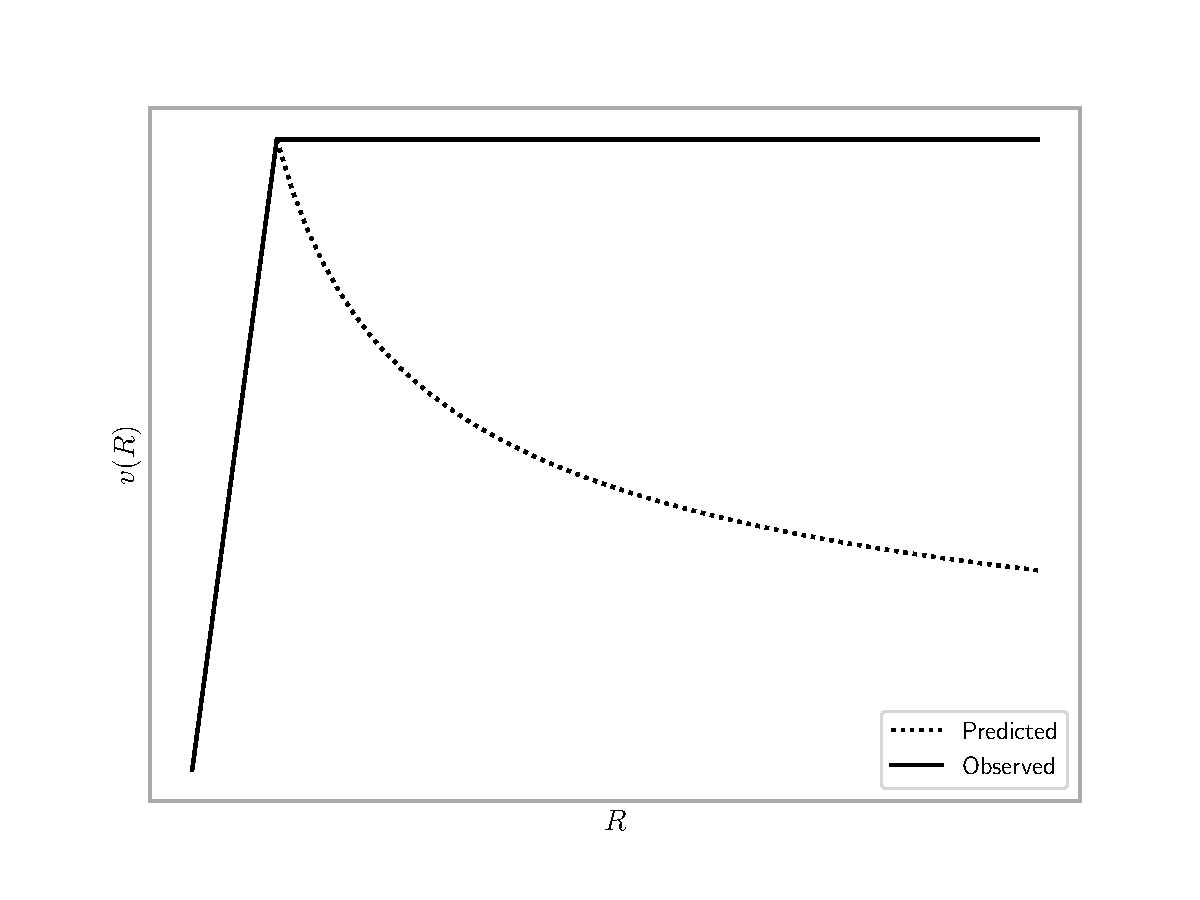
\includegraphics[width=\textwidth]{figures/Dark_matter.pdf}
\caption{Predicted and observed velocity distribution for galaxies. The point at which they star to diverge is approximately the radius of the bulk of the galaxy. This plot is approximate, realistic models do not have such sharp corners.}
\label{fig:dark_matter}
\end{figure}  

Instead of this, when in the 1980s people started to be able to measure this curve accurately they saw that, after the linear region, \(v(R)\) was approximately constant.
So, is Newtonian gravity wrong?

An option to solve this problem was proposed by Milgrom and collaborators: it is called MOdified Newtonian Dynamics, or MOND: they propose that gravity is not actually always described by a \(r^{-1}\) potential, but instead at low accelerations it behaves differently.
Specifically, they posit that the gravitational acceleration \(g\) should be modulated by a factor \(\mu (g / a_0 )\), where \(a_0 \approx \num{8e-10} h^2 \SI{}{m /s^2}\) is a characteristic acceleration while \(\mu (x)\) is an adimensional function such that \(\mu \rightarrow 1\) for \(x \gg 1\) and \(\mu \rightarrow x\) for \(x \ll 1\), such as \(\mu = x / (1+x)\) \cite{bekensteinDoesMissingMass1984}.

This approach is Newtonian but there are also relativistic MOND variants. They do not match observation as well as the alternative approach does.\footnote{MOND would be compatible with the speed of gravity being less than the speed of light, which is equivalent to the graviton being massive. Recent measurements of gravitational waves seem to agree with the general-relativistic prediction that it is massless.}
The heaviest thing weighing against MOND is the fact that even using it we still need dark matter in order to fully explain observations.

\subsubsection{Dark matter}

The alternative option is that Newtonian mechanics describes galactic mechanics well, but the galaxy's matter distribution inferred from our observations is actually smaller than the real distribution, which extends outward further than the matter we can see: this is \textbf{dark matter}.

We'd need mass obeying \(M (R) \propto R\) in order to have a constant value of \(v\): since \(M(R) = 4 \pi \int_0^{R_{\text{max}}}  R^2 \rho(R) \dd{R}\), we need the density profile to decay like \(\rho(R) \propto R^{-2}\).
This is called a \emph{thermal} density profile: we call it the \emph{dark matter halo}, which surrounds all spiral galaxies.

We do not know what dark matter is: we can say that it   interacts gravitationally but not electromagnetically.
People tend to believe that it is made up of beyond-the-standard-model particles, like a \emph{neutralino} or an \emph{axion}.
Historically, people thought the effect could be due to massive neutrinos; however their mass would need to be around \SI{30}{eV}, and the analysis of the CMB data showed that the sum of the masses of the neutrino species must be \(\sum m_\nu < \num{0.120}\) \cite[Table 7]{PlanckCollaboration:2018I}.

The total density of matter (dark+regular) is \(\sim 6\) times more than that of regular matter alone: this must be accounted for in our estimate of the \(M/L\) ratio for spiral galaxies (since we have additional mass but not additional luminosity):
with this correction, we find that for spiral galaxies
%
\begin{align}
\expval{\frac{M}{L}} \approx 300 h \frac{M_{\odot}}{L_{\odot}}
\,,
\end{align}
%

\subsubsection{Elliptical galaxies}

If galaxies are not spiral-shaped, we have to weigh them in a different way: the Doppler broadening of spectral lines gives us a measure of the root-mean-square velocity.

% \subsection{Virial theorem}
Later in the course we will obtain the (nonrelativistic) \emph{virial theorem}, now we just state it: if \(T\) is the kinetic energy of a gravitationally bound system, \(U\) is the potential energy, then
%
\begin{equation}
  2T + U = 0
\end{equation}
%
holds when the inertia tensor stabilizes, that is, when we have dynamical equilibrium.

The kinetic energy is \(T = \frac{3}{2} M \expval{v_r^2} \), where \(v_r\) is the radial\footnote{By ``radial'' we mean directed towards us, not towards the center of the galaxy.}
component of the velocity, which we expect to account for one third of total energy by the equipartition theorem.
\(M\) is the total mass of the galaxy.

The potential energy, instead, is \(U = - G M^2 /R\). Substituting these expressions into the virial theorem we get
%
\begin{align}
2 \times \frac{3}{2} M \expval{v_r^2} - \frac{GM^2}{R} &= 0  \\
M &= \frac{3R}{G} \expval{v_r^2}
\,,
\end{align}
%
so if we can measure \(\expval{v_r^2}\) through Doppler broadening and we can give a reasonable estimate for the radius \(R\) of the galaxy we can give an estimate for \(M\).

\subsubsection{Global matter contributions}

Accounting for the dark matter mass, we get \(\expval{M/L} \approx 300 h M_\odot / L_\odot\).

To date, the best estimate for \(\rho_{0c}\) is 
%
\begin{align}
\rho_{0c} \approx \num{1.88e-29} h^2 \SI{}{g /cm^3}
\,,
\end{align}
%
so, in order to have \(\Omega = 1\), we'd need \(\expval{M/L}\) to be equal to:
%
\begin{align}
\expval{\frac{M}{L}} 
= \frac{\rho_{0c}}{\mathscr{L}_{g}}
\approx \frac{\SI{1.88e-29}{\littleh^2 g /cm^{3}}}{\SI{2e8}{\littleh \Lsun /Mpc^{3}}}
\approx 1390 h M_{\odot} / L_{\odot}
\,.
\end{align}

% So measuring the number density of galaxies and their velocities we get a way to measure \(\Omega_0\).

We can define quantities of the form \(\Omega_{0i}  = \rho_{0i} / \rho_{0c}\), where \(i\) is a type of matter, such as baryonic matter, dark matter, dark energy, radiation and so on, whose density is represented as \(\rho_{0i}\).

These variables quantify how much, at the present, time, of the cosmic energy budget is accounted for by that type of matter.

So, only \(\Omega_{0b} \approx 5\%\) of the energy budget is given by baryonic matter (not all of which is visible), while around \(\Omega_{0 DM} \approx 27\%\) is dark matter.
Together, they are just denoted as ``matter'', and \(\Omega_{0m} \approx 30 \%\).

We can ask ourselves: is dark matter actually baryonic matter which for some reason we cannot see, such as black holes or brown dwarfs?

This cannot be the case: our observations, combined with models for primordial nucleosynthesis,
% \todo[inline]{Ricordati di mettere la referenza al paragrafo della nucleosintesi quando lo sistemerai, che sarebbe carino}
gives the following bounds for the baryonic energy density: 
%
\begin{equation}
0.013 \leq \Omega_{\text{0b}} h^2 \leq 0.025
\,.
\end{equation}

The upper bound for \(\Omega_{0b}\) is around \(2.5\%/h^2 \approx \SI{5.4}{\percent}\).

% where \(\Omega_b\) corresponds to the baryonic density: so the universe \emph{cannot} be made only of baryons.

% Dark matter likes ``clumping'': we characterize it by this property.

This would seem to indicate that \(\Omega_{0} \approx \num{.3} \ll 1\): however we are failing to consider a crucial contribution.
Consider the second Friedmann equation \eqref{eq:friedmann-2}: in the Newtonian limit \(P \sim 0\) while \( \rho >0 \), so we get \(\ddot{a} <0\): the universe contracts.
This is not what is observed: we actually see it in accelerated expansion.

\subsubsection{Dark energy}

The measurements leading to this conclusion are performed by estimating the distance and redshift of far-away objects whose intrinsic luminosity is well known, called \emph{standard candles}: the most commonly used are type Ia supernovae and Cepheid variables.

So, if the expansion is accelerated then \(\ddot{a} > 0\): this means, again from the second Friedmann equation \eqref{eq:friedmann-2}, that \(P < -\rho c^2/3\).
This is commonly expressed by defining \(w = P / \rho c^2\). 
In order to have accelerated expansion we need \(w < -1/3\); what is observed is closer to \(w \sim -1\).

This negative pressure has the effect of a \emph{tension}, pulling the universe apart.
This contribution is also called a ``cosmological constant term'', for reasons which will be expanded upon in later sections, and denoted with the letter \(\Lambda \).

We cannot see directly neither dark matter nor dark energy: how do we distinguish the two? Dark matter tends to cluster, while dark energy is uniformly distributed.

From observations of both the anisotropies in the CMB and the distribution of galaxies we can determine that \(\Omega_{\Lambda } \approx \num{.7}\).

% The Friedmann equation would imply deceleration if \(\rho, P \geq 0\): dark energy seems to have \emph{negative pressure}.

\subsubsection{Radiation}

We still need to compute the contribution of the energy of electromagnetic and neutrino radiation to the total energy balance.
Let us start with radiation: the greatest fraction of the radiation energy density is contained in the CMB, which is extremely close to a Planckian distribution: 
%
\begin{align}
B (\nu, T) = \frac{2 h}{c^2} \frac{\nu^3}{\exp(\frac{h \nu }{k_B T}) - 1}
\,,
\end{align}
%
with \(T = T_{0 \gamma } \approx \SI{2.725(1)}{K}\). \(B\) is a measure of spectral intensity: it is measured in units of energy per unit second, area, solid angle and frequency. This is a well-known distribution, whose integral is given by
%
\begin{equation}
  \rho_{0 \gamma} = \frac{\sigma_r T_{0 \gamma}^4}{c^2} = \SI{4.8e-34}{\gram\per\centi\metre\cubed}
\end{equation}
%
where \(\sigma_r = \pi^2 k_B^4 / (15 \hbar ^3 c^3)\), while \(\sigma_{SB} = \sigma_r c /4\).

\todo[inline]{Doing the computation, by }
\begin{lstlisting}[language=Python]
(4 * cosmo.Tcmb0**4 * ac.sigma_sb / ac.c**3 ).cgs
\end{lstlisting}
\todo[inline]{gives \SI{4.6e-34}{g / cm^3}: it is very close to the figure of 4.8 given in \cite{Pacciani:2018}, but I do not see where the discrepancy would come from. (Confermo il tuo conto, magari ha cacciato un typo)}

So, we have that the radiation contribution to the global energy balance is \(\Omega_{0 \gamma } \approx \SI{2.5e-5}{\littleh^{-2}} < \SI{.01}{\percent}\), definitely negligible.

\todo[inline]{Typo in \cite{Pacciani:2018}: exponent of \(h\) is \(-2\), not \(+2\).}

We are going to show in later sections
% \todo[inline]{Qui pure sarebbe carino mettere la ref alla sezione}
that if neutrinos were massless, their temperature would be \(T_\nu = (4/11)^{1/3} T_\gamma < T_\gamma \).

They might not be massless, and if they are not the main contribution to the energy density they will give will be from their masses.
However, recent observations (for example, by the Planck satellite) are bounding the mass of the neutrinos,
\(\sum m_\nu \leq \SI{0.12}{eV} \): we have 
%
\begin{equation}
\rho_\nu = 3 N_\nu \frac{\expval{m_\nu} }{\SI{10}{eV}} \SI{e-30}{\gram\per\cubic\centi\metre}
\,,
\end{equation}
%
where \(N_{\nu }\) is the number of neutrino species. 
Even if we assume the upper bound, \(N_{\nu } \expval{m_{\nu }} = \SI{.12}{eV}\), we get \(\Omega_{0 \nu } < \SI{.5}{\percent}\). 

\subsubsection{Conclusions}

% In the end we have \(\Omega = 1 = \Omega_b + \Omega_{DM} + \Omega_{DE}\) (do note that the value of 1 is measured, not theoretical!)
If we add up all the contributions to  \(\Omega = \Omega_b + \Omega_{DM} + \Omega_{\Lambda }\) (neglecting, as we said, the contributions by EM radiation and neutrinos) we find experimentally \(\Omega_{k} = \Omega-1 \approx (5^{+38}_{-40}) \times  \num{e-4}\) \cite[Table A.2]{planckcollaborationPlanck2018Results2019a}.

So, with the data we have currently we cannot determine the sign of the universe's spatial curvature.

\subsection{The Hubble law}

\begin{figure}[ht]
\centering
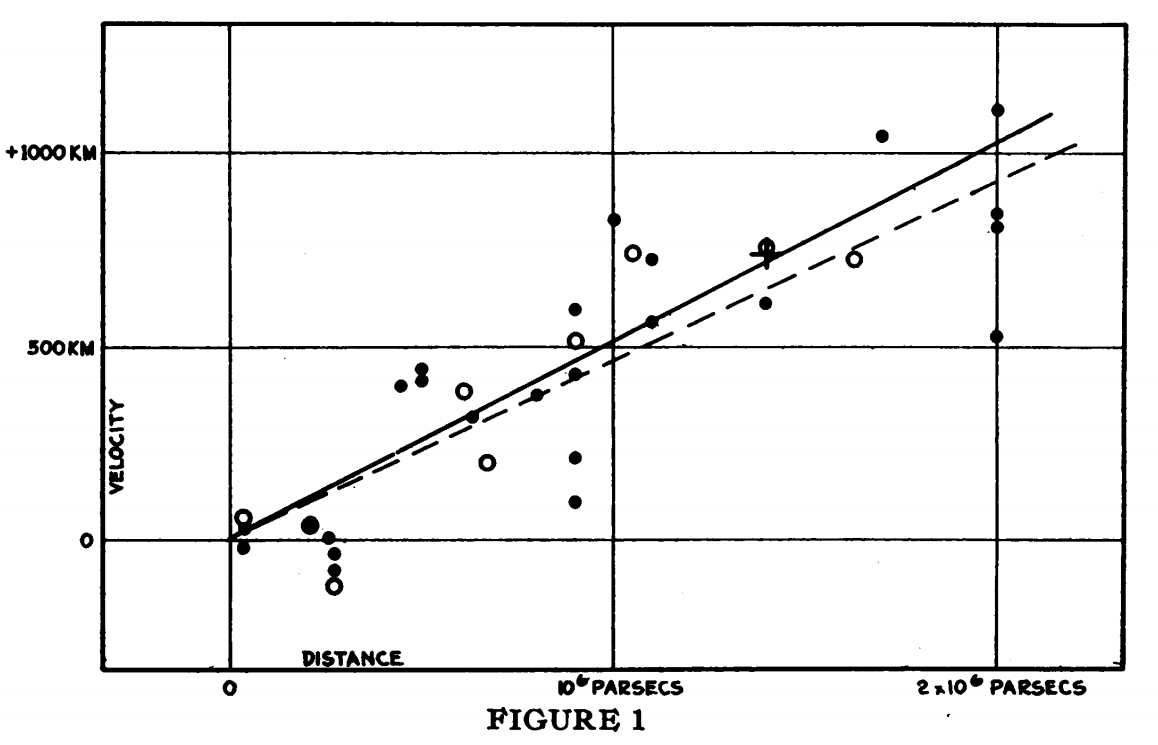
\includegraphics[width=\textwidth]{figures/hubble_original.png}
\caption{Original velocity versus distance data from Edwin Hubble's paper in 1929 \cite{hubbleedwinRelationDistanceRadial1929}.}
\label{fig:hubble_original}
\end{figure}

At the end of the 1920s Edwin Hubble compared the estimates for the distances of far-away galaxies (obtained through standard candles and other types of estimates) to their velocities relative to us, as measured through their redshift. His results are shown in figure \ref{fig:hubble_original}: he obtained a roughly linear relation in the form:
%
\begin{equation}
  v = H_0 d\,,
\end{equation}
%
where \(v\) is the velocity of the galaxies, and \(d\) is their distance from us, while \(H_0 \) is a constant of proportionality.
Hubble's measurements suggested \(H_0 \sim \SI{500}{km/s/Mpc}\), more refined modern ones using techniques similar to those used by Hubble yield a value of \SI{73.24(174)}{km/s/Mpc} \cite{riessDeterminationLocalValue2016}.

Measurements of \(H_0 \) through analysis of the CMB gives an incompatible value: \(H_0 = \SI{67.8(9)}{km/s/Mpc}\) \cite{PlanckCollaboration:2016XIII}.


Let us now show that this \(H_0 \) is actually the same one we defined before, \(H_0 = \dot{a} / a\).
\(H_0 \) is called the \textbf{Hubble constant}, since it is constant with respect to the direction we look in the sky.

% Can we derive this from the Robertson-Walker line element?
% It was actually derived first by Lemaitre.

We are considering the distance connecting us (the center of our reference frame) to a distance galaxy: so we drop the angular part in the flat (\(k = 0\)) Friedmann-Lemaître-Robertson-Walker (FLRW) line element:
%
\begin{equation}
  \dd{s^2} = c^2 \dd{t^2} - a^2(t) \dd{r^2}
\end{equation}

So, at a fixed time the physical distance is given by \(d = a(t) r\): therefore \(v = \dot{d} = \dot{a}r = \frac{\dot{a} }{a} d = H_0 d\). 

Do note that we neglected the temporal part of the metric: this is equivalent to assuming that photons travel instantaneously.
Assuming the universe is spatially flat is correct up to second order: for a general value of \(k\) we have 
%
\begin{align}
d = a \int_{0}^{r} \frac{ \dd{\widetilde{r}} }{\sqrt{1 - k \widetilde{r}^2}} = a  \qty( r + \mathcal{O}(r^3))
\,,
\end{align}
%
since the integral gives either \(r\), \(\arcsin(r)\) or \(\operatorname{arcsinh}(r)\), depending on \(k\) and all three of these equal \(r\) up to second order.

So, this is Newtonian and rough, but it gives us the correct intuitive idea.
We now wish to make this reasoning more precise.

The first step, since we want to discuss our observations of light, is to define the redshift.

\begin{definition}[Redshift]
The redshift \(z\) of a photon is defined by
%
\begin{equation}
  z = \frac{\lambda_0 - \lambda_e}{\lambda_{e}}
  = \frac{\lambda_0 }{\lambda_{e}} - 1
  = \frac{\nu_{e}}{\nu_{0}} - 1
  \,,
\end{equation}
%
where \(\lambda_0\) and \(\lambda_e\) are the observed and emission wavelengths respectively, while \(\nu \) are frequencies with the same notation.
\end{definition}

We will show
% \todo[inline]{Idem sarebbe bella la ref al punto dove viene dimostrato}
that the redshift can be found from the ratio of the scale factors now and at emission: \(1+z = a_0/ a_e\).
Therefore, \(\nu_o / \nu_e = a_e / a_0\).

We wish to study the distribution of light from an astronomical source: in Minkowski spacetime the apparent luminosity \(\ell\) decreases like \(r^{-2}\) if \(r\) is the distance from the object.
In a generic spacetime this will not be the case: however, we can define a measure of spatial distance \(d_L\) such that \(\ell = L / (4 \pi d_L^2)\), where \(L\) is the intrinsic luminosity of the object.

Do note that \(\ell \) is dimensionally a luminosity flux: it is measured in units of energy per unit time per unit area.

\begin{definition}  
The luminosity distance \(d_L\) is defined as:
%
\begin{equation}
d_L = \sqrt{\frac{L}{4 \pi \ell} } \,.
\end{equation}

Since \(L \propto \ell\), this is a well-defined measure of distance between two generic points in spacetime, regardless of the presence of a source of light there.
\end{definition}
  
How do we relate the luminosity distance and the scale factor?
The radiation from our source is spread on a sphere: we integrate the angular part of the FLRW metric over a sphere of fixed comoving radius \(r\) to find its area.

The metric restricted to the angular coordinates at fixed \(r\) is given by 
%
\begin{align}
\dd{s^2} = a^2 r^2 \qty(\dd{\theta^2} + \sin^2\theta \dd{\varphi^2})
\,,
\end{align}
%
so the area form on the surface of the sphere is 
%
\begin{align}
\dd{A} = \sqrt{ \det g} \dd{\theta } \wedge \dd{\varphi }
\,,
\end{align}
%
where \(\sqrt{ \det g} = \sqrt{a^{4} r^{4} \sin^2\theta } = a^2r^2 \sin \theta \). 
So,
%
\begin{align}
A = \int_{S^{2}}  \dd{A} = a^2r^2 \int_{0}^{\pi } \dd{\theta } \int_{0}^{2 \pi } \dd{\varphi } \sin \theta = 4 \pi a^2r^2 
\,,
\end{align}
%
where we substituted the wedge product for the regular tensor product of the differentials since our axes are orthogonal.
Now, at which time do we compute the scale factor? We are measuring the flux at the surface of the sphere, at the time at which we are observing: therefore we need to compute it at observation time. This gives us \(A = 4 \pi r^2a_0^2\).

Now, the emitted luminosity is in the form: 
%
\begin{align}
L = \dv{N}{t_{e}} \expval{h \nu_{e} }
\,,
\end{align}
%
where \(\dv*{N}{t}\) is the number of photons emitted per unit time, whose average energy is \(\expval{h \nu }\).
From the point of view of the observer, the number of photons is the same, while the frequency of the observed photon and the time interval \(\dd{t_{e}}\) change: specifically, \(\nu_{e} = \nu_0 a_0 / a_e\) and \(\dd{t_{e}} = \dd{t_0 } a_e / a_0 \).\footnote{This is the case even though the temporal component of the metric does not change, since we are not considering a fixed instance of cosmic time (which is unphysical): instead, we are considering the time intervals that the emitter and observed measure between the crests of a light wave sent from one to the other.}
Therefore, the observed absolute luminosity obeys the relation \(L= L_0 (a_0 / a_e)^2 \).

So, putting everything together we get:
%
\begin{equation}
  \ell = \frac{L_0 }{A} 
  = \frac{L}{4 \pi r^2 a_0 ^2} \qty(\frac{a_e}{a_0}) ^2
  \,,
\end{equation}
%
note that the value of \(k\) does not enter into the equation.
% The corrective factor comes from the frequency dependence of energy and the fact that power is energy over time, which also changes.

Therefore:
%
\begin{equation} \label{eq:luminosity-distance}
d_L = \sqrt{\frac{L}{4 \pi \ell}}
= \sqrt{\frac{4 \pi r^2a_0^2}{4 \pi } \qty(\frac{a_0}{a_e})^2}
= \frac{a_0^2}{a_e} r = a_0  (1+z) r\,.
\end{equation}

\end{document}
